%% Figure2

\begin{figure}
	\centering
	\hspace*{\fill}
	%\subfigure[]{\label{fig:graylesion}\includegraphics[width=0.22\textwidth]{GrayLevel_D606.eps}}
	%\subfigure[]{\label{fig:grayhist}\includegraphics[width=0.22\textwidth]{GrayHist_D606.eps}}
	\subfloat[Lesion appearance of the \textit{Z} channel. The white delineation corresponds to our segmentation results.]{\label{fig:pdfseg-a}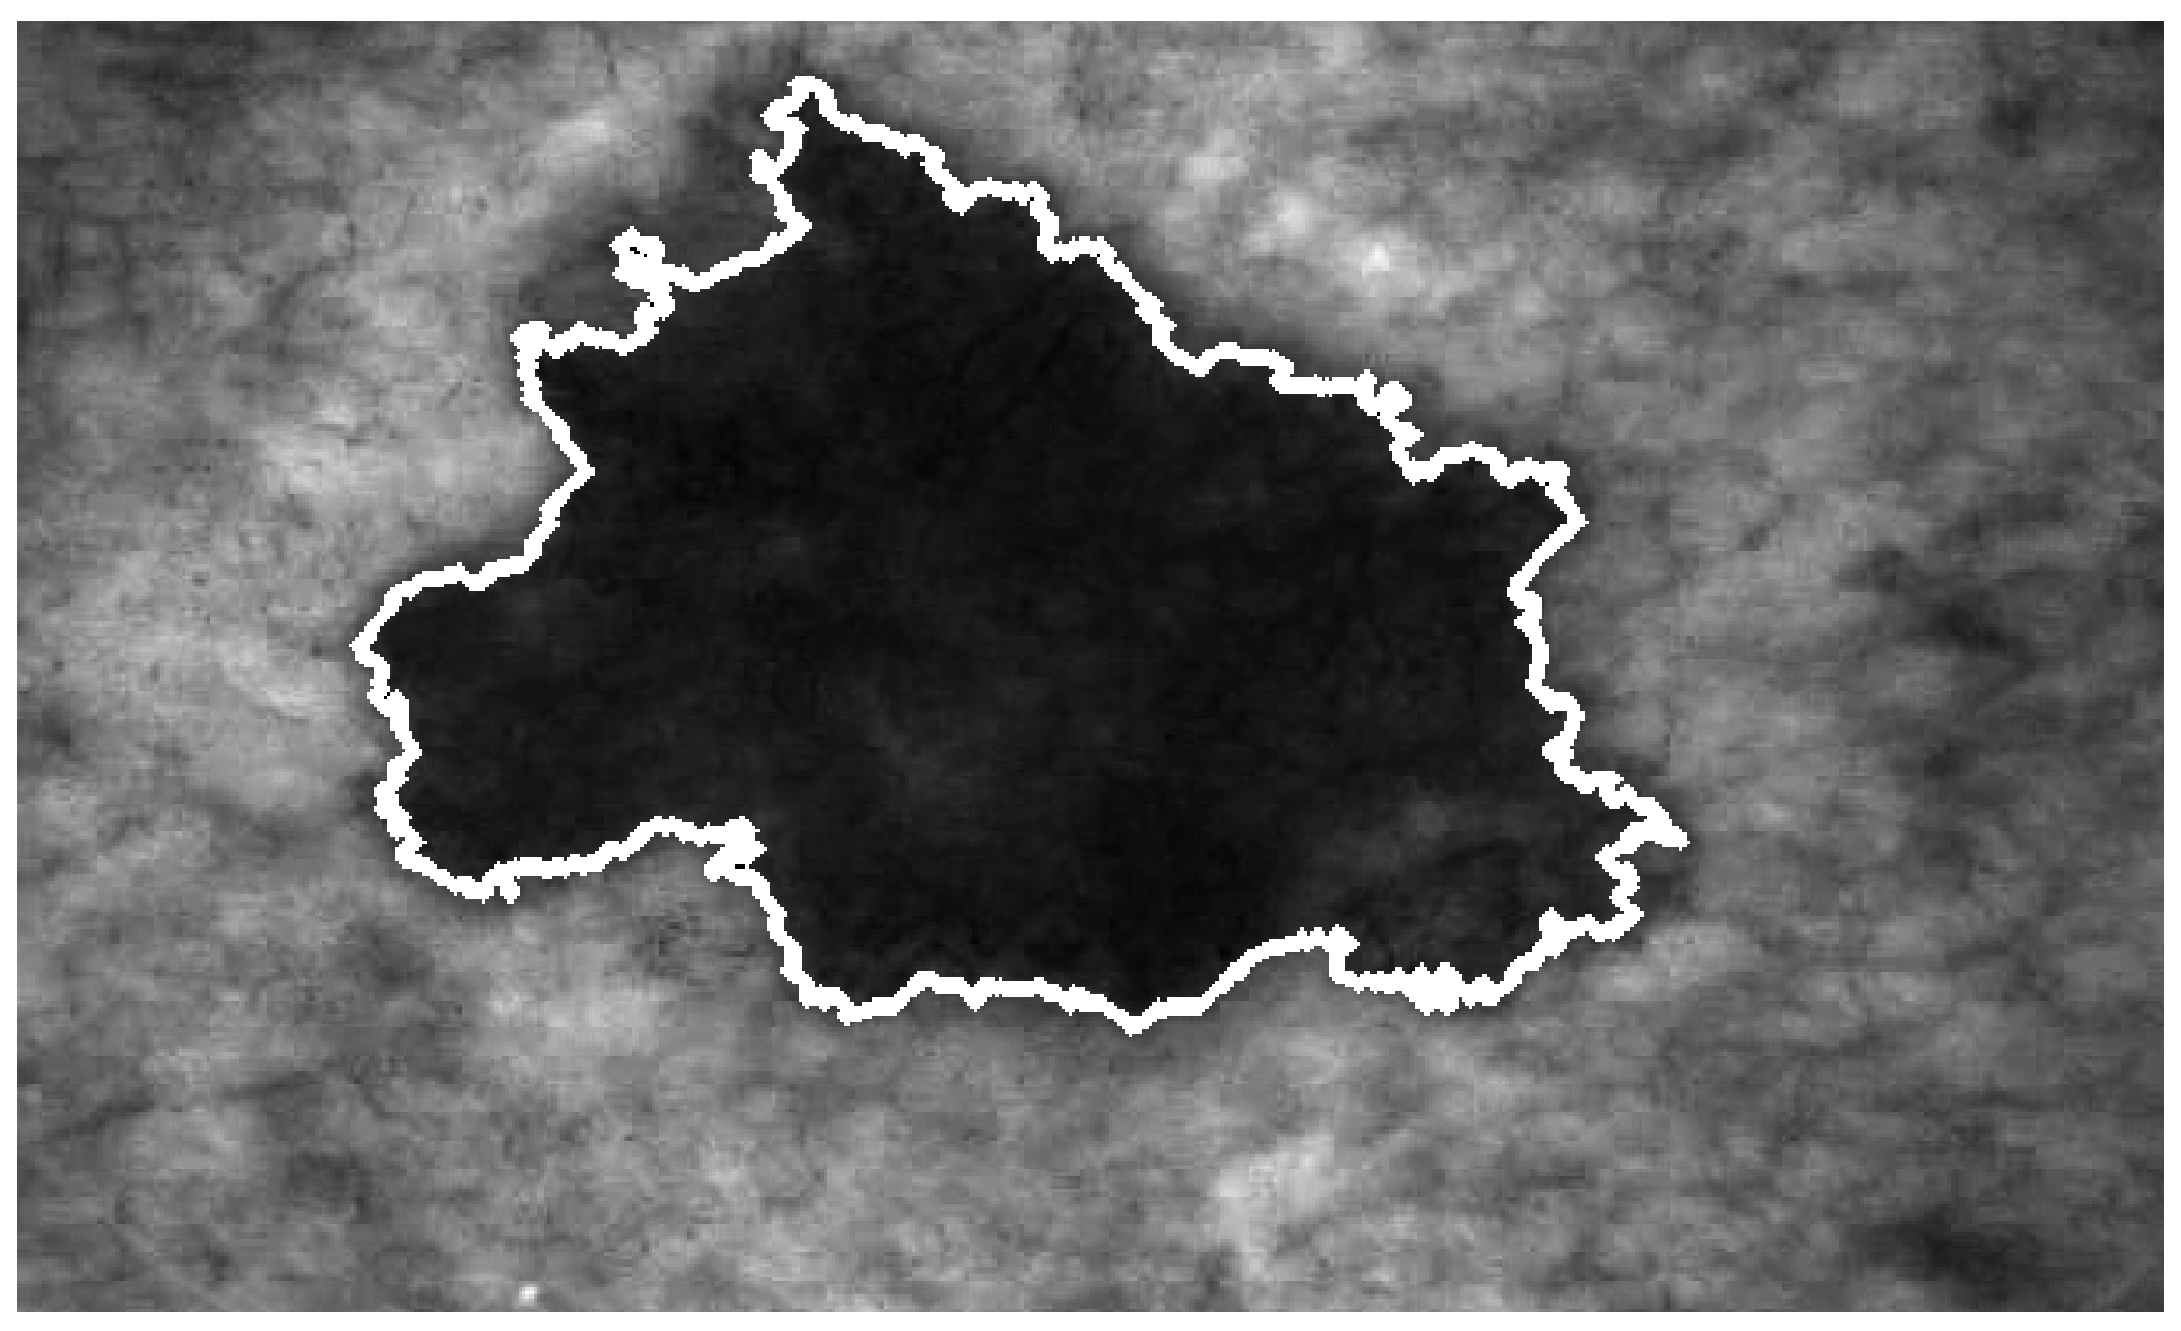
\includegraphics[height = 0.17\textheight, width=0.40\textwidth]{Chapter3/Figures/lesion_border.eps}}
	\hfill
	\subfloat[The \ac{pdf} corresponding to Fig \ref{fig:pdfseg-a}.]{\label{fig:pdfseg-b}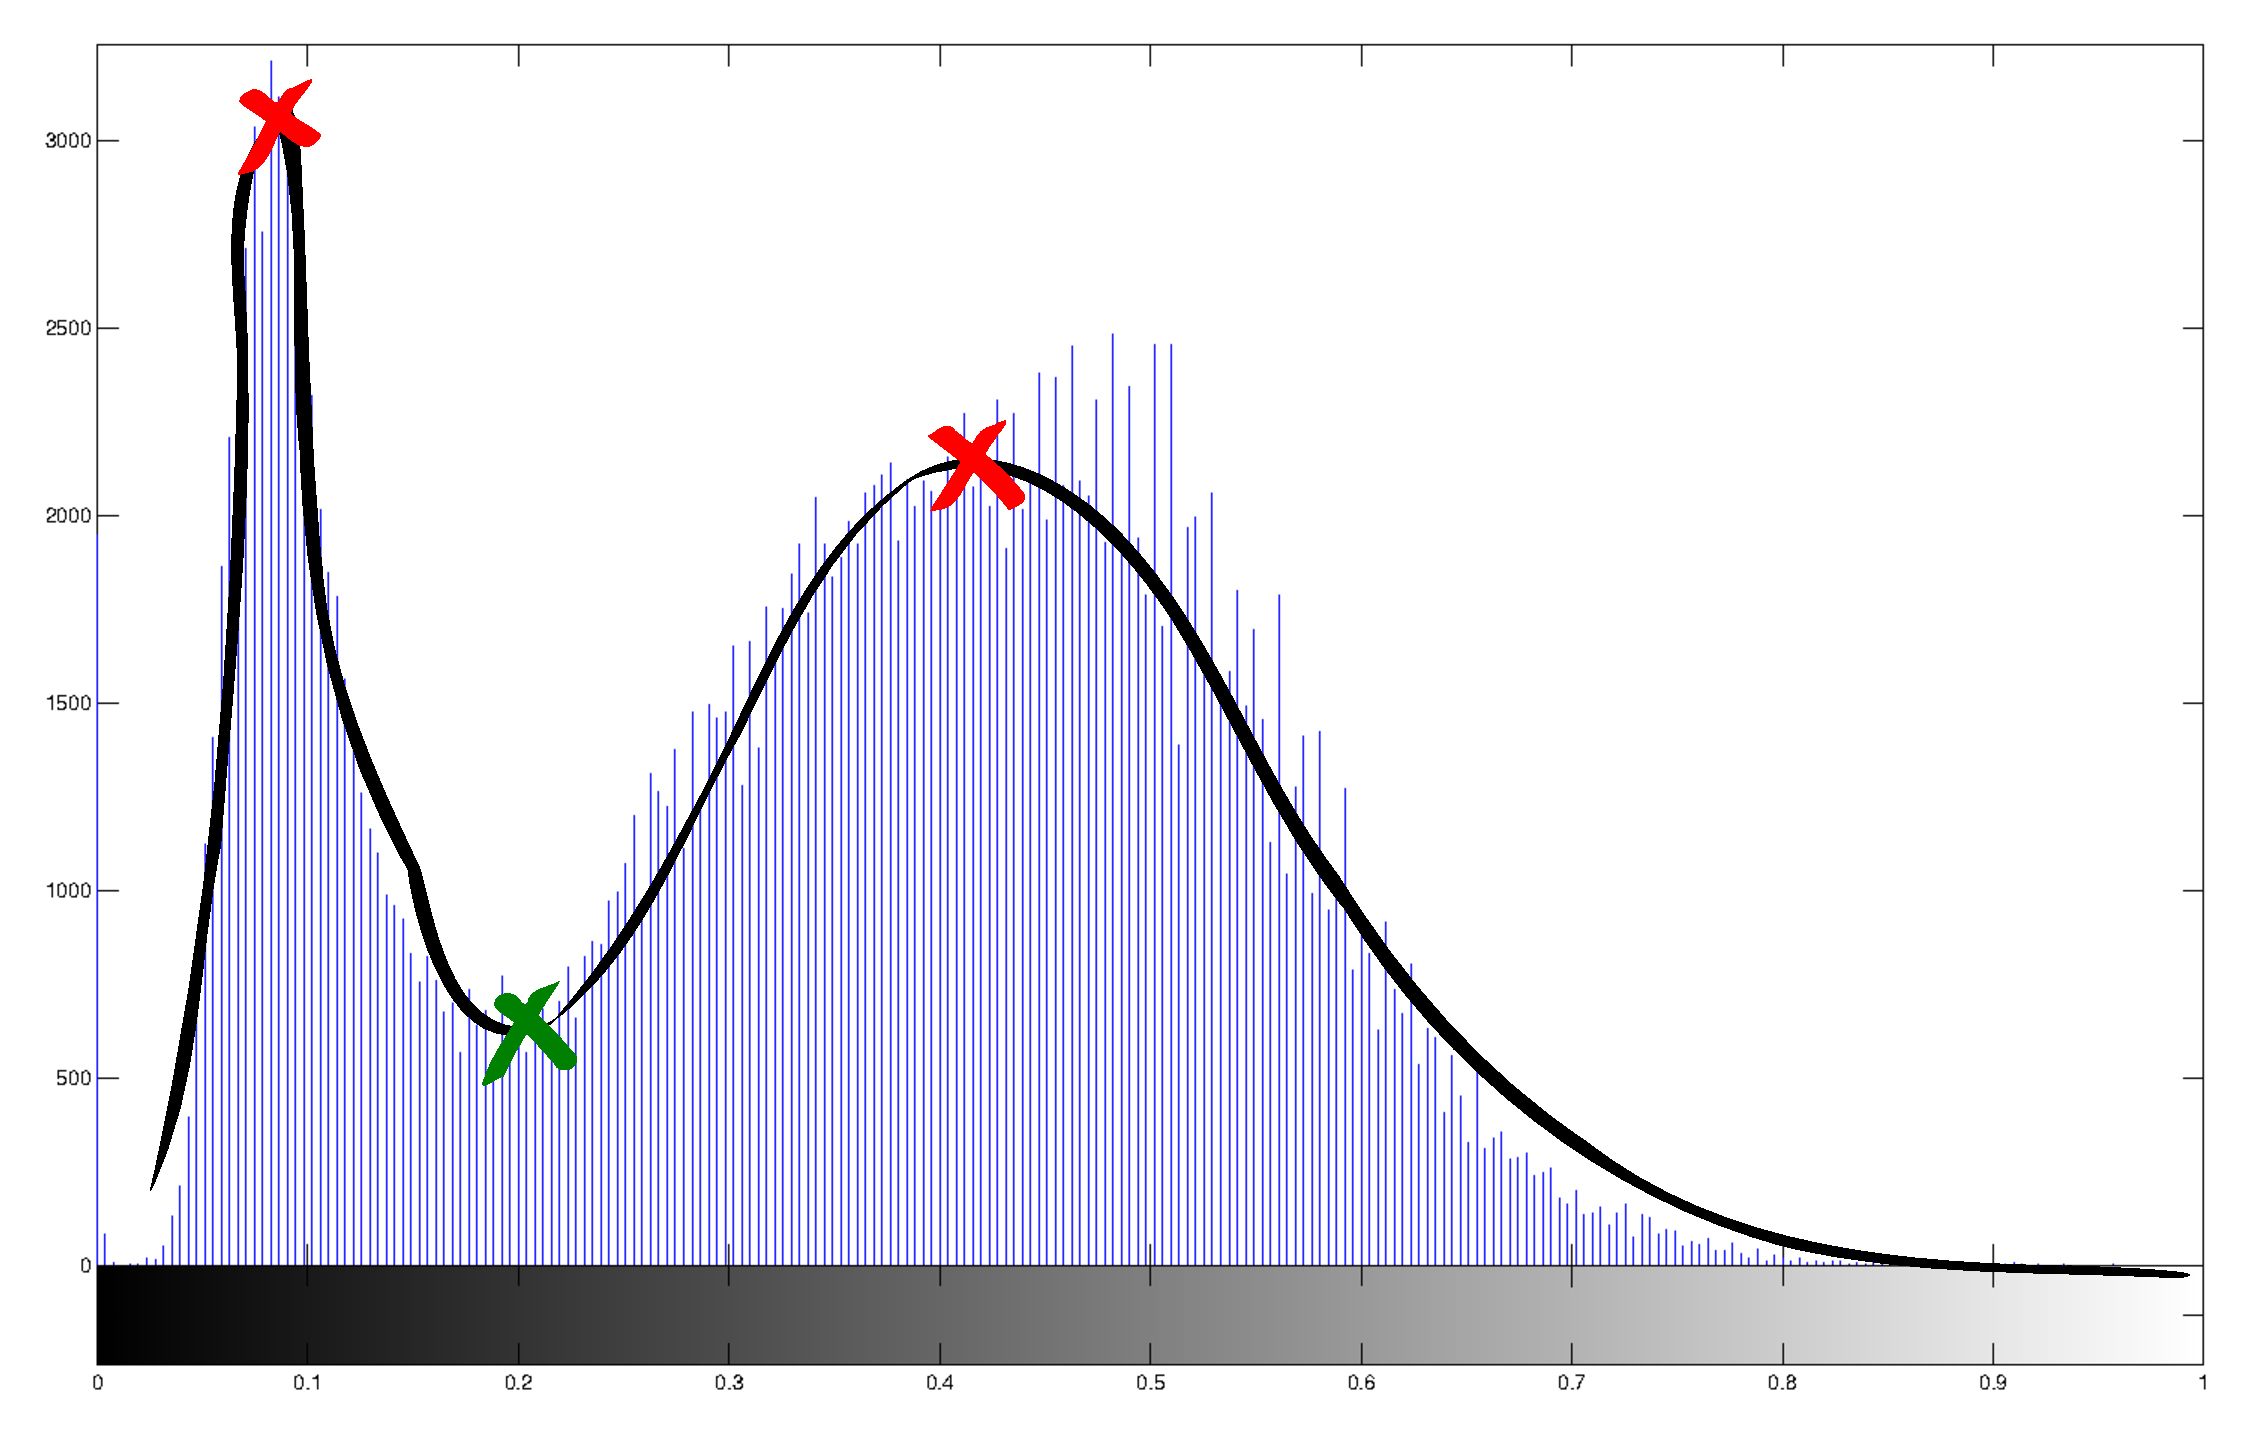
\includegraphics[ height = 0.17\textheight, width=0.40\textwidth]{Chapter3/Figures/ZNomrHist.eps}}
	\hspace*{\fill}
	\caption[\acl{pdf}-based segmentation]{Illustration of the \textit{Z} component (\textit{CIE XYZ} color space) of a dermoscopic image (a) with its corresponding \ac{pdf} (b). The distribution is characterized by a Gaussian mixture with two components. The best threshold is located at the valley between the two Gaussian bells (red cross between the the peaks).
The threshold in this case was found through the peak detetion algorithm and finding the local minium value.}
	\label{fig:pdfseg}
\end{figure}
